\documentclass[12pt]{article}
\usepackage[margin=1in]{geometry}
\usepackage{amsmath, amssymb, amsthm, graphicx, hyperref}
\usepackage{amsmath}
\usepackage{enumerate}
\usepackage{fancyhdr}
\usepackage{multirow, multicol}
\usepackage{tikz}
\usepackage{wrapfig}
\pagestyle{fancy}
\usepackage{titlesec}
\usepackage{lastpage}
\usepackage{multirow}
\usepackage{indentfirst}
\fancyhead[LO]{JACK Z}
\fancyhead[RO]{Page \thepage\ of \pageref{LastPage}}
\usepackage{comment}
\newtheorem{definition}{Definition}
\usepackage{amsmath}
\usepackage{booktabs}
\usepackage{xcolor}
\usepackage{tcolorbox}  % For creating styled boxes
\tcbuselibrary{most}
\usepackage{tcolorbox} % for creating colored or framed text boxes
\tcbuselibrary{breakable} % allows tcolorboxes to break across pages

\definecolor{examplebg}{RGB}{255, 228, 225} % Light red background
\tcbuselibrary{theorems} 
\usepackage{graphicx}
\usepackage{booktabs} % For better table formatting
\usepackage{caption} % Essential for \captionof
\usepackage{tcolorbox} % For creating colored boxes
\tcbuselibrary{most} % Load most libraries for tcolorbox

\newtcbtheorem[number within=subsection]{Note}{Note}{
    colback=Black!5,
    colframe=white!35!black,
    fonttitle=\bfseries,
    colbacktitle=blue!85!black,
    coltitle=white,
    enhanced,
    attach boxed title to top left={yshift=-2mm, xshift=2mm},
    boxed title style={sharp corners},
    sharp corners
}{Not}

\newtcbtheorem[number within=subsection]{Definition}{Definition}{
    colback=blue!5,
    colframe=blue!35!black,
    fonttitle=\bfseries,
    colbacktitle=blue!85!black,
    coltitle=white,
    enhanced,
    attach boxed title to top left={yshift=-2mm, xshift=2mm},
    boxed title style={sharp corners},
    sharp corners
}{def}

\newtcbtheorem[number within=subsection]{mytheorem}{Theorem}{
    colback=orange!5,      % Background color of the box
    colframe=orange,     % Border color of the box
    coltitle=white,     % Color of theorem title
    colbacktitle=orange!85!black,, % Background color for the title
    fonttitle=\bfseries,
    title after break={Theorem \csname the\tcbcounter\endcsname\ -- Continued}, % for continued theorems
    enhanced,
    attach boxed title to top left={yshift=-2mm, xshift=2mm},
    boxed title style={sharp corners, colframe=black},
    sharp corners,
    separator sign none % no sign between title and theorem text
}{thm}


\usepackage{lipsum} % 生成示例文本
\usepackage{fancyhdr}

\pagestyle{fancy}
\renewcommand{\headrulewidth}{0pt} % 去掉页眉下方的横线
\fancyfoot[C]{\textcopyright\ \fcolorbox{purple}{white}{Novel Prep}}

% Define custom colors
\definecolor{deepblue}{rgb}{0.0, 0.18, 0.39}
\definecolor{deepred}{rgb}{0.6, 0, 0}

% Define theorem style
\newtheoremstyle{beautifulthm}
  {10pt} % Space above
  {10pt} % Space below
  {\itshape} % Body font
  {} % Indent amount
  {\bfseries\color{deepblue}} % Theorem head font
  {.} % Punctuation after theorem head
  {.5em} % Space after theorem head
  {} % Theorem head spec

\theoremstyle{beautifulthm}
\newtheorem{theorem}{Theorem}[section]


\title{AP Calculus AB\&BC}
\author{Hongjun Zeng}
\maketitle

\lipsum[1-10] 

\newpage
\tableofcontents

\newpage

\begin{document}


\section{Limit}

\section{ Differentiation: Definition and Fundamental Properties}
\newpage
\subsection{The Derivative and the Tangent Line Problem}
\subsubsection{The Tangent Line Problem}
\begin{Definition}{Tangent Line with Slope \(m\)}{}
If \(f\) is defined on an open interval containing \(c\), and if the limit
\[
\lim_{\Delta x \to 0} \frac{\Delta y}{\Delta x} = \lim_{\Delta x \to 0} \frac{f(c + \Delta x) - f(c)}{\Delta x}
\]
exists, then the line passing through \((c, f(c))\) with slope \(m\) is the tangent line to the graph of \(f\) at the point \((c, f(c))\).

\begin{minipage}{\linewidth}
    \centering
    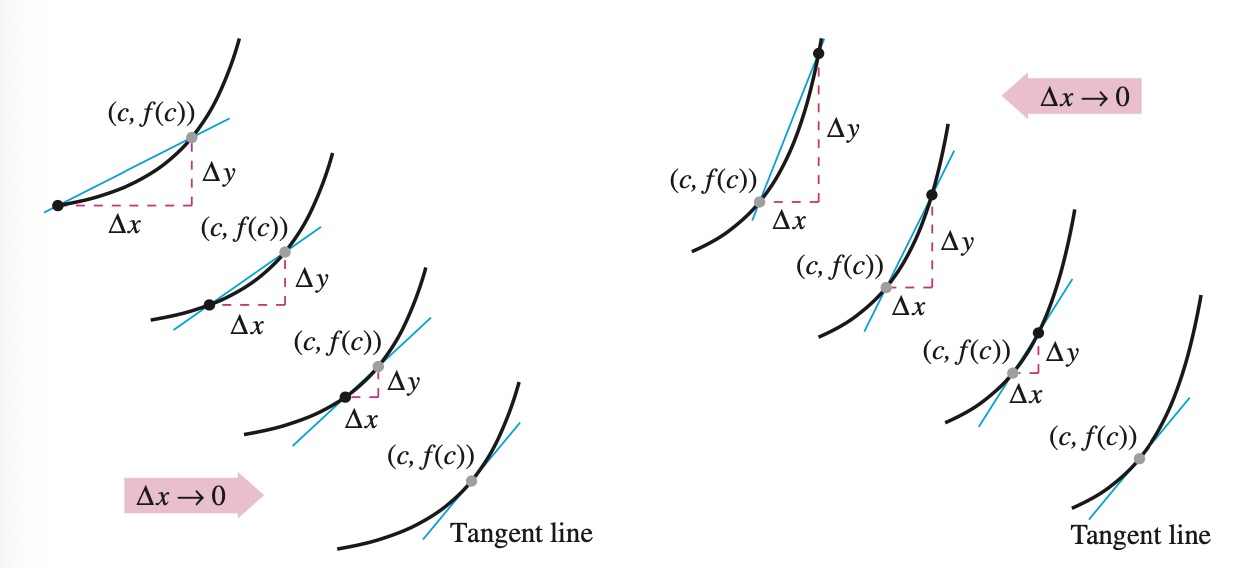
\includegraphics[width=0.80\linewidth]{Example_10.jpg} % Adjust the image width as necessary
    \captionof{figure}{}
    \label{fig:graph}
\end{minipage}
\end{Definition}
The slope of the tangent line to the graph of f at the point \((c, f(c))\)  is also called the slope of the graph of f at \(x = c\).




\begin{tcolorbox}[colback=examplebg, colframe=red!75!black, title=\textbf{EXAMPLE 1: The Slope of the Graph of a Linear Function}, fonttitle=\bfseries, sharp corners]
To find the slope of the graph of \(f(x) = 2x - 3\) when \(c = 2\), you can apply the definition of the slope of a tangent line, as shown.

\[
\lim_{\Delta x \to 0} \frac{f(2 + \Delta x) - f(2)}{\Delta x} = \lim_{\Delta x \to 0} \frac{[2(2 + \Delta x) - 3] - [2(2) - 3]}{\Delta x}
\]
\[
= \lim_{\Delta x \to 0} \frac{4 + 2\Delta x - 3 - 4 + 3}{\Delta x}
\]
\[
= \lim_{\Delta x \to 0} \frac{2\Delta x}{\Delta x}
\]
\[
= \lim_{\Delta x \to 0} 2
\]
\[
= 2
\]

This demonstrates that the slope of the line is indeed the coefficient of \(x\) in the linear equation \(f(x) = 2x - 3\), which is \(2\).

\end{tcolorbox}

\subsubsection{Rate of Change}
Suppose \(y\) is a quantity that depends on another quantity \(x\). Thus \(y\) is a function of \(x\) and we write \(y = f(x)\). If \(x\) changes from \(x_1\) to \(x_2\), then the change in \(x\) (also called the \textit{increment of \(x\)}) is:
\[
\Delta x = x_2 - x_1,
\]
and the corresponding change in \(y\) is:
\[
\Delta y = f(x_2) - f(x_1).
\]

The difference quotient:
\[
\frac{\Delta y}{\Delta x} = \frac{f(x_2) - f(x_1)}{x_2 - x_1},
\]
is called the \textbf{average rate of change of \(y\) with respect to \(x\)} over the interval \([x_1, x_2]\) and can be interpreted as the slope of the secant line \(PQ\)



\bigskip




\begin{Definition}{ Rate of Change}{}
The limit of these average rates of change is called the \textbf{(instantaneous) rate of change of \(y\) with respect to \(x\) at \(x = x_1\)}, which (as in the case of velocity) is interpreted as the slope of the tangent to the curve \(y = f(x)\) at \(P(x_1, f(x_1))\):
\[
\text{Instantaneous rate of change} = \lim_{\Delta x \to 0} \frac{\Delta y}{\Delta x} = \lim_{x_2 \to x_1} \frac{f(x_2) - f(x_1)}{x_2 - x_1}.
\]


\end{Definition}


\begin{tcolorbox}[colback=examplebg, colframe=red!75!black, title=\textbf{EXAMPLE 2:Understanding the Derivative in a Practical Context}, fonttitle=\bfseries, sharp corners]
A manufacturer produces bolts of fabric with a fixed width. The cost of producing \(x\) yards of this fabric is \(C = f(x)\) dollars.

\vspace{3mm}
\textbf{ What is the meaning of the derivative \(f'(x)\)? What are its units?}
\vspace{5mm}
\tcblower

\textbf{Solution:} The derivative \(f'(x)\) is the \textbf{instantaneous rate of change} of \(C\) with respect to \(x\); that is, \(f'(x)\) represents the rate of change of the production cost with respect to the number of yards produced. Economists refer to this rate of change as the \textbf{marginal cost}.

\[
f'(x) = \lim_{\Delta x \to 0} \frac{\Delta C}{\Delta x}.
\]

The units for \(f'(x)\) are the same as the units for the difference quotient \(\Delta C / \Delta x\). Since \(\Delta C\) is measured in dollars and \(\Delta x\) in yards, the units for \(f'(x)\) are \textbf{dollars per yard}.

\end{tcolorbox}




\newpage

\subsubsection{The Derivative of a Function}
\begin{Definition}{the Derivative of a Function}{}
The derivative of \(f\) at \(x\) is
\[
f'(x) = \lim_{\Delta x \to 0} \frac{f(x + \Delta x) - f(x)}{\Delta x}
\]
provided the limit exists. For all \(x\) for which this limit exists, \(f'\) is a function of \(x\).
\end{Definition}



\begin{tcolorbox}[colback=examplebg, colframe=red!75!black, title=\textbf{EXAMPLE 2: Finding the Derivative using the definition}, fonttitle=\bfseries, sharp corners]
Find the derivative of \(f(x) = x^3 + 2x\) using the definition
\tcblower
\textbf{Solution:}

Given \(f(x) = x^3 + 2x\), the derivative of \(f(x)\) using the definition is:
\[
f'(x) = \lim_{h \to 0} \frac{f(x + h) - f(x)}{h}.
\]

Substitute back into the formula:
\[
f'(x) = \lim_{h \to 0} \frac{(x^3 + 3x^2h + 3xh^2 + h^3) + 2x + 2h - x^3 - 2x}{h}.
\]

Simplify the numerator:
\[
f'(x) = \lim_{h \to 0} \frac{3x^2h + 3xh^2 + h^3 + 2h}{h}.
\]

Factor out \(h\) in the numerator:
\[
f'(x) = \lim_{h \to 0} \frac{h(3x^2 + 3xh + h^2 + 2)}{h}.
\]

Cancel \(h\) in the numerator and denominator:
\[
f'(x) = \lim_{h \to 0} (3x^2 + 3xh + h^2 + 2).
\]

Take the limit as \(h \to 0\):
\[
f'(x) = 3x^2 + 2.
\]

Thus, the derivative of \(f(x) = x^3 + 2x\) is:
\[
f'(x) = 3x^2 + 2.
\]
\end{tcolorbox}

\newpage
\subsubsection{Differentiability and Continuity}

The alternative limit form of the derivative shown below is useful in investigating the relationship between differentiability and continuity. The derivative of \(f\) at \(c\) is defined as:
\[
f'(c) = \lim_{x \to c} \frac{f(x) - f(c)}{x - c}
\]
provided this limit exists.

\begin{minipage}{\linewidth}
    \centering
    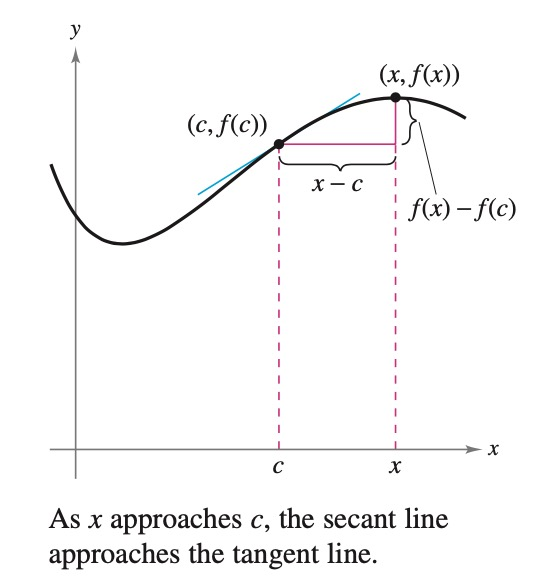
\includegraphics[width=0.550\linewidth]{Example_12.jpg} % Adjust the image width as necessary
    \captionof{figure}{}
    \label{fig:graph}
\end{minipage}

\begin{Definition}{Differentiability and Continuity}{}
A function \(f\) is \textbf{differentiable at \(a\)} if \(f'(a)\) exists. It is \textbf{differentiable on an open interval} \((a, b)\) [or \((a, \infty)\) or \((-\infty, a)\) or \((-\infty, \infty)\)] if it is differentiable at every number in the interval.
\end{Definition}

\textbf{How Can a Function Fail To Be Differentiable?}

A function \(f\) may fail to be differentiable at a point \(x = a\) in the following ways:

\begin{enumerate}
    \item \textbf{Corners or Kinks:} If the graph of \(f\) has a corner or kink at \(x = a\), the graph changes direction abruptly, and the left-hand derivative and right-hand derivative at \(a\) are not equal. 

    \item \textbf{Discontinuity:} If \(f\) is not continuous at \(x = a\), then \(f\) is not differentiable at \(a\). For example, jump discontinuities make the function non-differentiable.

    \item \textbf{Vertical Tangent Line:} If the graph of \(f\) has a vertical tangent line at \(x = a\), this implies that \(\lim_{x \to a} |f'(x)| = \infty\). In this case, the tangent lines become steeper and steeper as \(x\) approaches \(a\).

\end{enumerate}



\begin{minipage}{\linewidth}
    \centering
    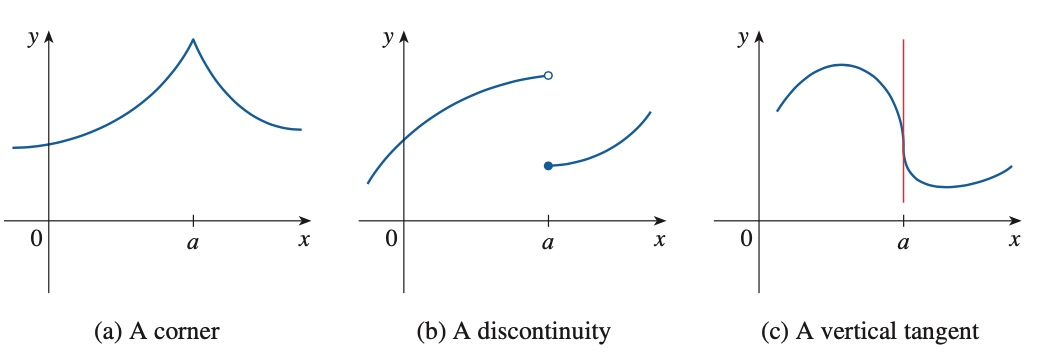
\includegraphics[width=0.90\linewidth]{Example_13.jpg} % Adjust the image width as necessary
    \captionof{figure}{}
    \label{fig:graph}
\end{minipage}

\begin{tcolorbox}[colback=examplebg, colframe=red!75!black, title=\textbf{EXAMPLE 3: A Graph with a Sharp Turn}, fonttitle=\bfseries, sharp corners]

The function \(f(x) = |x - 2|\), is continuous at \(x = 2\). The one-sided limits, however, are:

\[
\lim_{x \to 2^-} \frac{f(x) - f(2)}{x - 2} = \lim_{x \to 2^-} \frac{|x - 2| - 0}{x - 2} = -1 \quad \text{(Derivative from the left)},
\]

and

\[
\lim_{x \to 2^+} \frac{f(x) - f(2)}{x - 2} = \lim_{x \to 2^+} \frac{|x - 2| - 0}{x - 2} = 1 \quad \text{(Derivative from the right)}.
\]

These one-sided derivatives are not equal. Therefore, \(f\) is \textbf{not differentiable} at \(x = 2\), and the graph of \(f\) does not have a tangent line at the point \((2, 0)\).
\begin{minipage}{\linewidth}
    \centering
    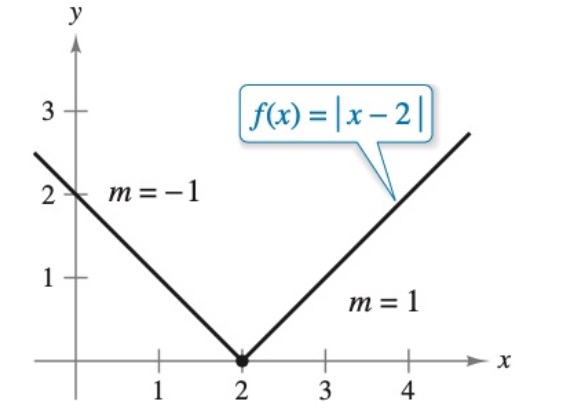
\includegraphics[width=0.50\linewidth]{Example_14.jpg} % Adjust the image width as necessary
    \captionof{figure}{}
    \label{fig:graph}
\end{minipage}


\end{tcolorbox}


\begin{tcolorbox}[colback=examplebg, colframe=red!75!black, title=\textbf{EXAMPLE 4: A Graph with a Vertical Tangent Line}, fonttitle=\bfseries, sharp corners]
The function \(f(x) = x^{1/3}\) is continuous at \(x = 0\), as shown in Figure 2.13. However, because the limit:
\[
\lim_{x \to 0} \frac{f(x) - f(0)}{x - 0} = \lim_{x \to 0} \frac{x^{1/3} - 0}{x} = \lim_{x \to 0} \frac{1}{x^{2/3}} = \infty,
\]
is infinite, you can conclude that the tangent line is vertical at \(x = 0\). So, \(f\) is \textbf{not differentiable} at \(x = 0\).

\begin{minipage}{\linewidth}
    \centering
    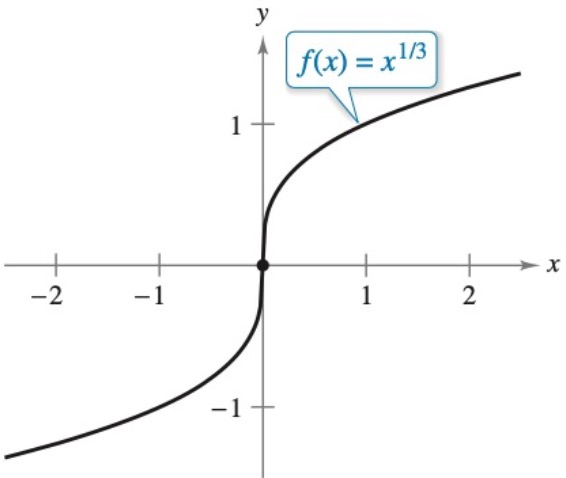
\includegraphics[width=0.50\linewidth]{Example_15.jpg} % Adjust the image width as necessary
    \captionof{figure}{}
    \label{fig:graph}
\end{minipage}

\bigskip

From these two examples, you can see that a function is not differentiable at a point at which its graph has a sharp turn \textbf{or} a vertical tangent line.


\end{tcolorbox}







\newpage
\subsection{Basic Differentiation Rules}
\subsubsection{The Constant Rule}
\begin{mytheorem}{The Constant Rule}{}
The derivative of a constant function is 0. That is, if \( c \) is a real number, then
\[
\frac{d}{dx}[c] = 0.
\]
\end{mytheorem}


\begin{tcolorbox}[colback=examplebg, colframe=red!75!black, title=\textbf{EXAMPLE 1: Using the Constant Rule}, fonttitle=\bfseries, sharp corners]
a. \( y = 7 \) \rightarrow \( \frac{dy}{dx} = 0 \) \\
b. \( f(x) = 0 \) \rightarrow \( f'(x) = 0 \) \\
c. \( s(t) = -3 \) \rightarrow \( s'(t) = 0 \) \\
d. \( y = k\pi^2, k \text{ is constant} \) & \( y' = 0 \)

\end{tcolorbox}


\subsubsection{Power Rule}
\begin{mytheorem}{Power Rule}{}
\textit{If \( n \) is a rational number, then the function \( f(x) = x^n \) is differentiable and}
\[ \frac{d}{dx}[x^n] = nx^{n-1}. \]

\textit{For \( f \) to be differentiable at \( x = 0 \), \( n \) must be a number such that \( x^{n-1} \) is defined on an interval containing 0.}
\end{mytheorem}

\begin{tcolorbox}[colback=examplebg, colframe=red!75!black, title=\textbf{EXAMPLE 2: Using the Power Rule}, fonttitle=\bfseries, sharp corners]
a. \( f(x) = x^3 \) \rightarrow \( f'(x) = 3x^2 \) \\
b. \( g(x) = x^{1/3} \) \rightarrow \( g'(x) = \frac{1}{3}x^{-2/3} = \frac{1}{3x^{2/3}} \) \\
c. \( y = \frac{1}{x^2} \) \rightarrow \( \frac{dy}{dx} = \frac{d}{dx}[x^{-2}] = (-2)x^{-3} = -\frac{2}{x^3} \) \\

\end{tcolorbox}

\subsubsection{The Constant Multiple Rule}
\begin{mytheorem}{The Constant Multiple Rule}{}
\textit{If \( f \) is a differentiable function and \( c \) is a real number, then \( cf \) is also differentiable and}
\[
\frac{d}{dx}[cf(x)] = c f'(x).
\]
\end{mytheorem}

\begin{tcolorbox}[colback=examplebg, colframe=red!75!black, title=\textbf{EXAMPLE 3: Using the Constant Multiple Rule}, fonttitle=\bfseries, sharp corners]
\begin{align*}
\textbf{Function} && \textbf{Derivative} \\
y = 5x^3 && \frac{dy}{dx} = 15x^2 \\
y = \frac{2}{x} && \frac{dy}{dx} = -\frac{2}{x^2} \\
f(t) = \frac{4t^2}{5} && f'(t) = \frac{8t}{5} \\
y = 2\sqrt{x} && \frac{dy}{dx} = \frac{1}{\sqrt{x}} \\
y = \frac{1}{2^{2/3}x^{1/2}} && \frac{dy}{dx} = -\frac{1}{3x^{5/3}} \\
y = -\frac{3x}{2} && y' = -\frac{3}{2}
\end{align*}

\end{tcolorbox}

\subsubsection{The Sum and Difference Rules}
\begin{mytheorem}{The Sum and Difference Rules}{}

The sum (or difference) of two differentiable functions \(f\) and \(g\) is itself differentiable. Moreover, the derivative of \(f + g\) (or \(f - g\)) is the sum (or difference) of the derivatives of \(f\) and \(g\).

\begin{align*}
\frac{d}{dx}[f(x) + g(x)] &= f'(x) + g'(x) & \text{(Sum Rule)} \\
\frac{d}{dx}[f(x) - g(x)] &= f'(x) - g'(x) & \text{(Difference Rule)}
\end{align*}
\end{mytheorem}

\begin{tcolorbox}[colback=examplebg, colframe=red!75!black, title=\textbf{EXAMPLE 4: Using the Sum and Difference Rules}, fonttitle=\bfseries, sharp corners]
\begin{itemize}
    \item[\textbf{a.}] For the function \( f(x) = x^3 - 4x + 5 \), the derivative is:
    \[
    f'(x) = 3x^2 - 4
    \]

    \item[\textbf{b.}] For the function \( g(x) = -\frac{x^4}{2} + 3x^3 - 2x \), the derivative is:
    \[
    g'(x) = -2x^3 + 9x^2 - 2
    \]

    \item[\textbf{c.}] For the function \( y = \frac{3x^2 - x + 1}{x} = 3x - 1 + \frac{1}{x} \), the derivative is:
    \[
    y' = 3 - \frac{1}{x^2} = \frac{3x^2 - 1}{x^2}
    \]
\end{itemize}

\end{tcolorbox}


\subsubsection{Derivatives of Sine and Cosine Functions}
\begin{mytheorem}{Derivatives of Sine and Cosine Functions}{}

The derivatives of the sine and cosine functions are given by:
\[
\frac{d}{dx}[\sin x] = \cos x
\]
\[
\frac{d}{dx}[\cos x] = -\sin x
\]
\end{mytheorem}


\begin{tcolorbox}[colback=examplebg, colframe=red!75!black, title=\textbf{EXAMPLE 5: Derivatives of Sine and Cosine Functions}, fonttitle=\bfseries, sharp corners]
\begin{enumerate}
    \item[a.] $y = 2 \sin x$
    \[
    y' = 2 \cos x
    \]
    \item[b.] $y = \frac{\sin x}{2} = \frac{1}{2} \sin x$
    \[
    y' = \frac{1}{2} \cos x
    \]
    \item[c.] $y = x + \cos x$
    \[
    y' = 1 - \sin x
    \]
    \item[d.] $y = \cos x - \frac{\pi}{3} \sin x$
    \[
    y' = -\sin x - \frac{\pi}{3} \cos x
    \]
\end{enumerate}

\end{tcolorbox}

\newpage
\subsection{ Product and Quotient Rules and Higher-Order Derivatives}

In the previous section, you learned that the derivative of the sum of two functions is simply the sum of their derivatives. The rules for the derivatives of the product and quotient of two functions are not as simple.
\subsubsection{Product Rule}
\begin{mytheorem}{Product Rule}{}

If \( f \) and \( g \) are both differentiable, then:
\[
\frac{d}{dx} [f(x)g(x)] = f(x) \frac{d}{dx} [g(x)] + g(x) \frac{d}{dx} [f(x)]
\]
\end{mytheorem}

\begin{tcolorbox}[colback=examplebg, colframe=red!75!black, title=\textbf{EXAMPLE 1: Using the Product Rule}, fonttitle=\bfseries, sharp corners]
Differentiate the function \( f(t) = \sqrt{t} (a + bt) \).

\tcblower
\textbf{Solution:}

Using the Product Rule, we have:
\[
f'(t) = \sqrt{t} \frac{d}{dt} (a + bt) + (a + bt) \frac{d}{dt} (\sqrt{t})
\]
\[
= \sqrt{t} \cdot b + (a + bt) \cdot \frac{1}{2} t^{-1/2}
\]
\[
= b\sqrt{t} + \frac{a + bt}{2\sqrt{t}} = \frac{a + 3bt}{2\sqrt{t}}
\]

\end{tcolorbox}

\newpage

\subsubsection{Quotient Rule}
\begin{mytheorem}{Quotient Rule}{}

If \( f \) and \( g \) are differentiable, then:
\[
\frac{d}{dx} \left[ \frac{f(x)}{g(x)} \right] = \frac{g(x) \frac{d}{dx} [f(x)] - f(x) \frac{d}{dx} [g(x)]}{[g(x)]^2}
\]
\end{mytheorem}

\begin{tcolorbox}[colback=examplebg, colframe=red!75!black, title=\textbf{EXAMPLE 2: Using the Quotient Rule}, fonttitle=\bfseries, sharp corners]

Find an equation of the tangent line to the curve \( y = \frac{e^x}{1 + x^2} \) at the point \( \left(1, \frac{1}{2}e\right) \).

\tcblower
\textbf{Solution:}

According to the Quotient Rule, we have:
\[
\frac{dy}{dx} = \frac{(1 + x^2) \frac{d}{dx}(e^x) - e^x \frac{d}{dx}(1 + x^2)}{(1 + x^2)^2}
\]
\[
= \frac{(1 + x^2)e^x - e^x(2x)}{(1 + x^2)^2}
\]
\[
= \frac{e^x(1 - 2x + x^2)}{(1 + x^2)^2}.
\]

So the slope of the tangent line at \( \left(1, \frac{1}{2}e\right) \) is:
\[
\left. \frac{dy}{dx} \right|_{x=1} = 0.
\]

This means that the tangent line at \( \left(1, \frac{1}{2}e\right) \) is horizontal and its equation is:
\[
y = \frac{1}{2}e.
\]

\end{tcolorbox}




\begin{Note}{Table of Differentiation Formulas}{}

\[
\frac{d}{dx}(c) = 0 \quad \frac{d}{dx}(x^n) = nx^{n-1} \quad \frac{d}{dx}(e^x) = e^x
\]


\[
(cf)' = cf' \quad (f+g)' = f' + g' \quad (f-g)' = f' - g'
\]


\[
(fg)' = f'g + g'f \quad \left( \frac{f}{g} \right)' = \frac{gf' - fg'}{g^2}
\]

\end{Note}


\newpage
\subsection{Derivatives of Trigonometric Functions}

\setlength{\tabcolsep}{1em}

\begin{Note}{Table of  Trigonometric Functions}{}
\[
\begin{aligned}
    \frac{d}{dx}(\sin x) & = \cos x \hspace{2cm} \frac{d}{dx}(\csc x) = -\csc x \cot x \\
    \frac{d}{dx}(\cos x) & = -\sin x \hspace{2cm} \frac{d}{dx}(\sec x) = \sec x \tan x \\
    \frac{d}{dx}(\tan x) & = \sec^2 x \hspace{2cm} \frac{d}{dx}(\cot x) = -\csc^2 x
\end{aligned}
\]
\end{Note}

\begin{tcolorbox}[colback=examplebg, colframe=red!75!black, title=\textbf{EXAMPLE 1: Derivatives of Trigonometric Functions}, fonttitle=\bfseries, sharp corners]

Differentiate \(f(x) = \frac{\sec x}{1 + \tan x}\). For what values of \(x\) does the graph of \(f\) have a horizontal tangent?

\tcblower
\textbf{Solution:}

The Quotient Rule gives:

\[
f'(x) = \frac{(1 + \tan x) \frac{d}{dx}(\sec x) - \sec x \frac{d}{dx}(1 + \tan x)}{(1 + \tan x)^2}
\]

Substituting the derivatives:

\[
f'(x) = \frac{(1 + \tan x)(\sec x \tan x) - \sec x (\sec^2 x)}{(1 + \tan x)^2}
\]

Simplify the numerator:

\[
f'(x) = \frac{\sec x (\tan x + \tan^2 x - \sec^2 x)}{(1 + \tan x)^2}
\]

Using the Pythagorean identity \(\sec^2 x = 1 + \tan^2 x\):

\[
f'(x) = \frac{\sec x (\tan x - 1)}{(1 + \tan x)^2}
\]

Thus, the derivative is:

\[
f'(x) = \frac{\sec x (\tan x - 1)}{(1 + \tan x)^2}
\]
\end{tcolorbox}



\begin{tcolorbox}[colback=examplebg, colframe=red!75!black, title=\textbf{EXAMPLE 2: Derivatives of Trigonometric Functions}, fonttitle=\bfseries, sharp corners]

Find the 27th derivative of \(\cos x\).

\tcblower
\textbf{Solution:}
The first few derivatives of \(f(x) = \cos x\) are as follows:

\[
f'(x) = -\sin x
\]
\[
f''(x) = -\cos x
\]
\[
f'''(x) = \sin x
\]
\[
f^{(4)}(x) = \cos x
\]
\[
f^{(5)}(x) = -\sin x
\]

We see that the successive derivatives occur in a cycle of length 4, and in particular,
\[
f^{(n)}(x) = \cos x \quad \text{whenever } n \text{ is a multiple of 4.}
\]

Therefore,
\[
f^{(24)}(x) = \cos x
\]

And, differentiating three more times, we have:
\[
f^{(27)}(x) = \sin x
\]

\end{tcolorbox}

\end{document}